\documentclass{report}
\usepackage{fancyhdr} % Required for custom headers
\usepackage{lastpage} % Required to determine the last page for the footer
\usepackage{extramarks} % Required for headers and footers
\usepackage{graphicx} % Required to insert images
%\usepackage{lipsum} % Used for inserting dummy 'Lorem ipsum' text into the template
\usepackage{amsmath}
\usepackage{float}
\usepackage{graphicx} 
%\usepackage{amsfont}
%\usepackage{amssymb}

\usepackage{multicol}
% Margins
\topmargin=-0.5in
\evensidemargin=0in
\oddsidemargin=-0.5in
\textwidth=7.5in
\textheight=9.0in
\headsep=0.25in 


\pagestyle{fancy}

%\rhead{\textbf{Marshall's Recipes}} % Top right header
%\lhead{\textbf{Curry Stir Fry}}
%\chead{ }
%\title{Curry Stir Fry}

\begin{document}
%\vspace{8mm}
%\textbf{PRELIMINARIES:}


\bigskip

\bigskip

\begin{multicols}{2}
\textbf{Ingredients}
\begin{itemize}
\item 3.5 cups flour \quad (1596 kCal/ 49 gP/ 4 gF/ 336 gC)
\item 1 cup vegetable oil (1984 kCal/ 0 gP/ 224 gF/ 0 gC)
\item 3 eggs  \quad (234 kCal/ 18 gP/ 15 gF/ 3 gC)
\item 1 cup white sugar (774 kCal/ 0 gP/ 0 gF/ 200 gC)
\item 1 cup brown sugar \quad (551 kCal/ 0 gP/ 0 gF/ 142 gC)
\item 2 cups grated zucchini \quad (38 kCal/ 3 gP/ 1 gF/ 7 gC)
\item 3 teaspoons vanilla extract 
\item 1 tablespoon ground cinnamon
\item 1 teaspoon baking powder
\item 1 teaspoon baking soda 
\item 1 teaspoon salt
\item $\frac{1}{2}$ teaspoon nutmeg



\end{itemize}


\columnbreak
\textbf{Procedure:}
\medskip


\begin{enumerate}
\item Preheat oven to 325 degrees and grease and flour two $8\times4$ bread pans.


\medskip
\item Sift flour, salt, baking powder, baking soda, and cinnamon together in a bowl. 
\medskip

\item Beat eggs, oil, vanilla extract, and sugar in a large bowl. Add sifted ingredients to creamed mixture and beat well. Stir in zucchini and pour batter into prepared pans. 
\newline 

 \item Bake for 40-60 minutes, or until tester inserted in the middle comes out clean. Cool in pan on rack for 20 minutes. Remove bread from pan and let cool.   
\end{enumerate}
\begin{table}[H]
  \begin{center}
    \caption{Macro totals}
    \label{tab:table1}
    \begin{tabular}{c|c|c|c} % <-- Alignments: 1st column left, 2nd middle and 3rd right, with vertical lines in between
      \textbf{Calories} & \textbf{Protein} & \textbf{Fat} & \textbf{Carbs}\\
      \hline
      5,177 kCal & 70 g & 244 g & 688 g\\
    \end{tabular}
  \end{center}
\end{table}
\end{multicols}



%\begin{center}
%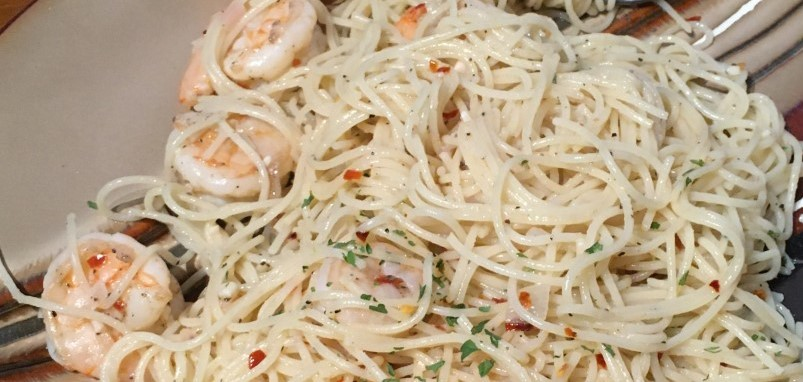
\includegraphics[scale=0.65]{Pasta/Shrimp Scampi/Shrimp Scampi.jpg}
%\end{center}


\end{document}